% Copyright 2021 Joel Feldman, Andrew Rechnitzer and Elyse Yeager, except where noted.
% This work is licensed under a Creative Commons Attribution-NonCommercial-ShareAlike 4.0 International License.
% https://creativecommons.org/licenses/by-nc-sa/4.0/


 \begin{frame}{Table of Contents }
\mapofcontentsC{\ce}
 \end{frame}
%%----------------------------------------------------------------------------------------
%%----------------------------------------------------------------------------------------
\section{3.5 Power series}
%---------------------------------------------------------------------------------------%----------------------------------------------------------------------------------------
\begin{frame}[t]
Recall the geometric series: for a constant $r$, with $|r|<1$:
\begin{align*}
\sum_{n=0}^\infty r^n & = \frac{1}{1-r}
\end{align*}
We can think of this as a function. If we set
\[f(x)=\sum_{n=0}^\infty x^n\]
and restrict our domain to $-1<x<1$, then 
\[f(x)=\sum_{n=0}^\infty x^n=\frac{1}{1-x}\]
\end{frame}
%----------------------------------------------------------------------------------------
\begin{frame}
\StatusBar{1}{5}

\centering
\begin{tikzpicture}
\myaxis{x}{3.5}{3.5}{y}{0}{5}
\draw[dashed](3,.5)--(3,4.5);
\xcoord{-3}{-1} \xcoord{3}{1}
\draw[thick,C1] plot[domain=-1:0.8,smooth]({\x*3},{1/(1-\x)})node[right]{$y=f(x)=\sum\limits_{n=0}^\infty x^n$};
\draw[C1](-3,.5)node[vertex,fill=white,draw]{};
\onslide<2|handout:0>{
	\color{W1}
	\xcoord{1.5}{\frac12}
	\draw(3/2,2)node[vertex]{};
	\ycoord{2}{2}
	\draw[<-](2,2)--+(.5,0)node[right,inner sep=0,fill=white]{$f\left(\frac12\right)=\sum\limits_{n=0}^\infty \left(\frac12\right)^n$};
	}
\onslide<3|handout:0>{
	\xcoord{3/5}{\frac15}
	\draw(3/5,5/4)node[vertex]{};
	\ycoord{5/4}{\frac54}
	\draw[<-](1.5,5/4)--+(.5,0)node[right,inner sep=0,fill=white]{$f\left(\frac15\right)=\sum\limits_{n=0}^\infty \left(\frac15\right)^n$};
	}
\onslide<4|handout:0>{
	\xcoord{-2.25}{-\frac34}
	\draw(-9/4,4/7)node[vertex]{};
	\ycoord{4/7}{\frac47}
	\draw[<-](1,4/7)--+(.5,0)node[right,inner sep=0,fill=white]{$f\left(-\frac34\right)=\sum\limits_{n=0}^\infty \left(-\frac34\right)^n$};
	}

\end{tikzpicture}
\end{frame}
%----------------------------------------------------------------------------------------
\begin{frame}[t]
\StatusBar{1}{6}
Why would we ever prefer to write $\sum\limits_{n=0}^\infty x^n$ instead of $\frac{1}{1-x}$?\pause\vfill

The function \[\sum_{n=0}^\infty x^n=1+x+x^2+x^3+x^4+\cdots\] isn't a polynomial, but in certain ways it behaves like one.
For $|x|<1$:
\pause\vfill

\begin{align*}
\diff{}{x}\left\{ \frac{1}{1-x}\right\}&\onslide<4->{=\diff{}{x}\sum_{n=0}^\infty x^n=\sum_{n=0}^\infty\left(\diff{}{x}\left\{x^n\right\}\right)=\sum_{n=0}^\infty nx^{n-1}\\[2em]}
\onslide<5->{\int\frac{1}{1-x} \ \dee x}\onslide<6->{ & = \int\left(\sum_{n=0}^\infty x^n \right) \dee x=\sum_{n=0}^\infty \left(\int x^n \ \dee x\right)
=\sum_{n=0}^\infty \frac{x^{n+1}}{n+1}}
\end{align*}
\vfill
\end{frame}
%----------------------------------------------------------------------------------------
\begin{frame}[t]
\unote{Definition~\eref{text}{def:SRpowerSeries}}
\begin{block}{Definition}
A series of the form
\begin{equation*}
 \sum_{n=0}^\infty A_n(x-c)^n=A_0 +A_1(x-c) + A_2(x-c)^2 + A_3 (x-c)^3 + \cdots
\end{equation*}
is called a \textit{power series in $(x-c)$} or a
\textit{power series centered on $c$}. The numbers $A_n$ are called
the coefficients of the power series.\\[1em]

One often considers power series centered on $c=0$ and then the series
reduces to
\begin{equation*}
 A_0 +A_1 x + A_2 x^2 + A_3 x^3 + \cdots
=\sum_{n=0}^\infty A_n x^n
\end{equation*}
\end{block}
\end{frame}
%----------------------------------------------------------------------------------------
\begin{frame}[t]
\NoSpace<2>\AnswerSpace
\begin{equation*}
 \sum_{n=0}^\infty A_n(x-c)^n=A_0 +A_1(x-c) + A_2(x-c)^2 + A_3 (x-c)^3 + \cdots
\end{equation*}
In a power series, we think of the coefficients $A_n$ as fixed constants, and we think of $x$ as the variable of a function.
\pause\medskip

Evaluate the power series $\sum\limits_{n=0}^\infty A_n(x-c)^n$ when $x=c$ :\medskip

\sonslide<3->{
\begin{align*} \sum_{n=0}^\infty A_n(x-c)^n&=A_0 +A_1(x-c) + A_2(x-c)^2 + A_3 (x-c)^3 + \cdots\\
\sum_{n=0}^\infty A_n(c-c)^n&=A_0 +A_1\underbrace{(c-c)}_0 + A_2\underbrace{(c-c)^2}_0 + A_3 \underbrace{(c-c)^3}_0 + \cdots\\
&=A_0 \text{ \quad (In particular, the series converges when $x=c$.)}
\end{align*}
}
\end{frame}
%----------------------------------------------------------------------------------------
\begin{frame}[t]
\only<1-2>{\AnswerYes}
\only<1>{\QuestionBar{1}{2}}
\only<2->{\AnswerBar{1}{2}}

A fundamental question we want to ask when we see a series is whether it converges or diverges. So, let's find all values of $x$ for which the power series
\[\sum_{n=1}^\infty \frac{x^n}{n} = x+\frac{x^2}{2}+\frac{x^3}{3}+\frac{x^4}{4}+\cdots\]
converges.\vfill

\sonly<2>{
This looks somewhat like a geometric series, but not exactly, so the ratio test is a good option.
\begin{align*}
\lim_{n \to \infty}\left|\frac{a_{n+1}}{a_n}\right|&=
\lim_{n \to \infty}\left|\frac{\frac{x^{n+1}}{n+1}}{\frac{x^n}{n}}\right|
=\lim_{n \to \infty} \left|\frac{x^{n+1}}{x^n}\right|\left(\frac{n}{n+1}\right)
\\&=\lim_{n \to \infty} \left|x\right|\left(\frac{n}{n+1}\right)=|x|
\end{align*}
So the series converges when $|x|<1$ and diverges when $|x|>1$. 
}
\sonly<3>{When $x=1$, we have the harmonic series, which diverges. When $x=-1$, we have the alternating harmonic series, which converges.\\[1em]

So, all together, the series converges when $-1 \le x <1$, and diverges everywhere else.
\begin{center}
\begin{tikzpicture}
\draw[<->] (-2,0)--(2,0);
\xcoord{1}{1}
\xcoord{-1}{-1}
\xcoord{0}{0}
\draw[line width=1mm, opacity=0.5] (-1,0)--(1,0);
\draw(-1,0)node[vertex]{};
\draw(1,0)node[vertex,fill=white,draw]{};
\end{tikzpicture}
\end{center}}

\snshonly{4}{2}{2}{\unote{Definition~\eref{text}{def:SRintervalofconvergence}}

\begin{block}{Definition}
Consider the power series
\begin{align*}
  \sum_{n=0}^\infty A_n (x-c)^n.
\end{align*}
The set of real $x$-values for which it converges is called the interval
of convergence of the series.
\end{block}}
\end{frame}
%----------------------------------------------------------------------------------------
\begin{frame}[t]
\AnswerYes<1-2>
\QuestionBar<1>{2}{2}
\AnswerBar<2->{2}{2}

Find the interval of convergence of the power series
\[\sum_{n=0}^\infty 2^n(x-1)^n = 
1+2(x-1)+2^2(x-1)^2+2^3(x-1)^3+\cdots~.
\]
\vfill

\sonly<2>{
This still looks somewhat like a geometric series, so the ratio test is a still good option to start.
\begin{align*}
\lim_{n \to \infty}\left|\frac{a_{n+1}}{a_n}\right|&=
\lim_{n \to \infty}\left|\frac{2^{n+1}(x-1)^{n+1}}{2^n(x-1)^n}\right|
=\lim_{n \to \infty} \left|\frac{(x-1)^{n+1}}{(x-1)^n}\right|\left(\frac{2^{n+1}}{2^n}\right)
\\&= 2\left|x-1\right|
\end{align*}
So we see that the series converges when $|x-1|<\frac12$ and diverges when $|x-1|>\frac12$. 
}
\sonly<3>{\small

When $x-1=-\frac12$, i.e. $x=\frac12$, our series is
\[\sum_{n=0}^\infty 2^n\left(\frac12-1\right)^n=
\sum_{n=0}^\infty 2^n \left(-\frac12\right)^n = 
\sum_{n=0}^\infty (-1)^n\]


When $x-1=\frac12$, i.e. $x=\frac32$, our series is
\[\sum_{n=0}^\infty 2^n\left(\frac32-1\right)^n=
\sum_{n=0}^\infty 2^n \left(\frac12\right)^n = 
\sum_{n=0}^\infty 1\]

In both cases, the series diverge by the divergence test. All together, the interval of convergence is ${\frac12 < x < \frac32}$.


\begin{center}
\begin{tikzpicture}
\draw[<->] (-2,0)--(2,0);
\xcoord{1}{3/2}
\xcoord{-1}{1/2}
\xcoord{0}{1}
\draw[line width=1mm, opacity=0.5] (-1,0)--(1,0);
\draw(-1,0)node[vertex,fill=white,draw]{};
\draw(1,0)node[vertex,fill=white,draw]{};
\end{tikzpicture}
\end{center}
}

\end{frame}
%----------------------------------------------------------------------------------------
\begin{frame}[t]
\AnswerYes<2>
\nsAnswerYes<2>
What happens if we apply the ratio test to a generic power series, $\sum\limits_{n=0}^\infty A_n(x-c)^n$?\pause
\begin{align*}
\lim_{n \to \infty}\left|\frac{A_{n+1}(x-c)^{n+1}}{A_n(x-c)^n}\right|&=
\lim_{n \to \infty}\left|\frac{A_{n+1}}{A_n}(x-c)\right|
=|x-c|\lim_{n \to \infty} \left| \frac{A_{n+1}}{A_n}\right|
\end{align*}
\begin{itemize}
\item If $\left| \frac{A_{n+1}}{A_n}\right|$ does not approach a limit as $n \to \infty$, the ratio test tells us nothing. (We should try other tests.)

\item If $\lim\limits_{n \to \infty} \left| \frac{A_{n+1}}{A_n}\right|=0$, then
 \onslide<3-|handout:0>{ \textcolor{spoilercolor}{the series converges for all $x$.}}

\item  If $\lim\limits_{n \to \infty} \left| \frac{A_{n+1}}{A_n}\right|=\infty$, then \onslide<3-|handout:0>{\textcolor{spoilercolor}{ the series converges when $x=c$, and diverges otherwise.}}

\item If $\lim\limits_{n \to \infty} \left| \frac{A_{n+1}}{A_n}\right|=A$ for some real number $A$, then
\onslide<3-|handout:0>{ \textcolor{spoilercolor}{the series converges when $|x-c|<\frac1A$, and diverges for $|x-c|>\frac1A$.\\ The cases $|x-c|=\frac1A$ need further inspection.}}



\end{itemize}
\end{frame}
%----------------------------------------------------------------------------------------
\begin{frame}[t]
\unote{Definition~\eref{text}{def:SRradiusConvergence}}
\begin{block}{Definition: Radius of Convergence}
\begin{enumerate}[(a)]
\item
Let $0<R<\infty$. If $\sum\limits_{n=0}^\infty A_n(x-c)^n$
converges for $|x-c|<R$,  and diverges for $|x-c| > R$,
then we say that the series has radius of convergence $R$.

\begin{center}
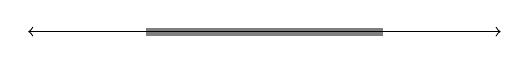
\begin{tikzpicture}
\draw[<->] (-3,0)--(3,0);
\xcoord{1.5}{c+R}
\xcoord{-1.5}{c-R}
\xcoord{0}{c}
\draw[line width=1mm, opacity=0.5] (-1.5,0)--(1.5,0);
\end{tikzpicture}
\end{center}
\item
If $\sum_{n=0}^\infty A_n(x-c)^n$ converges for every number $x$,
we say that the series has an infinite radius of convergence.
\begin{center}
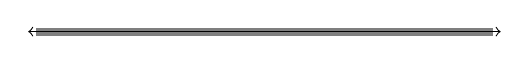
\begin{tikzpicture}
\draw[<->] (-3,0)--(3,0);
\xcoord{0}{c}
\draw[line width=1mm, opacity=0.5] (-2.9,0)--(2.9,0);
\end{tikzpicture}
\end{center}
\item
If $\sum_{n=0}^\infty A_n(x-c)^n$ diverges for every $x\ne c$,
we say that the series has radius of convergence zero.
\begin{center}
\begin{tikzpicture}
\draw[<->] (-3,0)--(3,0);
\xcoord{0}{c}
\draw(0,0)node[vertex]{};
\end{tikzpicture}
\end{center}
\end{enumerate}
\end{block}
\end{frame}
%----------------------------------------------------------------------------------------
\begin{frame}[t]
\sStatusBar{1}{4}
\AnswerYes<1-3>
\nsAnswerYes<1-3>
\begin{itemize}[<+->]
\item We saw that $\sum\limits_{n=0}^\infty x^n$ converges when $|x|<1$ and diverges when $|x|>1$, so this series has radius of convergence $R=\onslide<2-|handout:0>{\textcolor{spoilercolor}{1.}}$
\begin{center}
\begin{tikzpicture}
\draw[<->] (-2,0)--(2,0);
\xcoord{1}{1}
\xcoord{-1}{-1}
\xcoord{0}{0}
\draw[line width=1mm, opacity=0.5] (-1,0)--(1,0);
\draw(-1,0)node[vertex,fill=white,draw]{};
\draw(1,0)node[vertex,fill=white,draw]{};
\end{tikzpicture}
\end{center}
%
\item We saw that $\sum\limits_{n=1}^\infty \dfrac{x^n}{n}$ converges when $|x|<1$ and diverges when $|x|>1$, so this series also has radius of convergence $R=\onslide<3-|handout:0>{\textcolor{spoilercolor}{1.}}$
\begin{center}
\begin{tikzpicture}
\draw[<->] (-2,0)--(2,0);
\xcoord{1}{1}
\xcoord{-1}{-1}
\xcoord{0}{0}
\draw[line width=1mm, opacity=0.5] (-1,0)--(1,0);
\draw(-1,0)node[vertex]{};
\draw(1,0)node[vertex,fill=white,draw]{};
\end{tikzpicture}
\end{center}
%
\item We saw that $\sum\limits_{n=1}^\infty 2^n(x-1)^n$ converges when $|x-1|<\frac12$ and diverges when $|x-1|>\frac12$, so this series has radius of convergence $R=\onslide<4-|handout:0>{\textcolor{spoilercolor}{\frac12.}}$
\begin{center}
\begin{tikzpicture}
\draw[<->] (-2,0)--(2,0);
\xcoord{.5}{\frac32}
\xcoord{-.5}{\frac12}
\xcoord{0}{1}
\draw[line width=1mm, opacity=0.5] (-.5,0)--(.5,0);
\draw(-.5,0)node[vertex,fill=white,draw]{};
\draw(.5,0)node[vertex,fill=white,draw]{};
\end{tikzpicture}
\end{center}
\end{itemize}
\end{frame}
%----------------------------------------------------------------------------------------
\begin{frame}[t]
\AnswerSpace
\QuestionBar<1>{1}{2}\AnswerYes<1>
\AnswerBar<2->{1}{2}
\unote{Example~\eref{text}{eg:PWRb}}

What is the radius of convergence for the series $\sum\limits_{n=0}^\infty \frac{x^n}{n!}$ ?\\[1em]
\textit{Recall:}  $n!=(n)(n-1)(n-2) \cdots (2)(1)$.

\sonslide<2->{
\begin{align*}
\lim_{n \to \infty} \left|\frac{\frac{x^{n+1}}{(n+1)!}}{\frac{x^n}{n!}}\right|
&=\lim_{n \to \infty} \left|\frac{x^{n+1}}{x^n}\right| \frac{n!}{(n+1)!}
\\&=\lim_{n \to \infty} |x| \frac{(n)(n-1)(n-2) \cdots (2)(1)}{(n+1)(n)(n-1)(n-2)\cdots(2)(1)}\\
&=\lim_{n \to \infty}\frac{|x|}{n+1}=0
\end{align*}
For every real $x$, the limit is less than one, so the series converges. That is, its radius of convergence is $\infty$.
\begin{center}
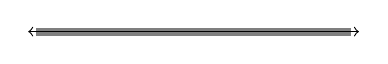
\begin{tikzpicture}
\draw[<->] (-2.1,0)--(2.1,0);
\xcoord{0}{0}
\draw[line width=1mm, opacity=0.5] (-2,0)--(2,0);
\end{tikzpicture}
\end{center}
}
\end{frame}
%----------------------------------------------------------------------------------------
\begin{frame}[t]
\AnswerSpace
\QuestionBar<1>{2}{2}\AnswerYes<1>
\AnswerBar<2->{2}{2}

\unote{Example~\eref{text}{eg:PWRda}, mostly}

What is the radius of convergence for the series $\sum\limits_{n=0}^\infty n! \cdot  (x-3)^n$ ?

\sonslide<2->{
\begin{align*}
\lim_{n \to \infty} \left|\frac{(n+1)!(x-3)^{n+1}}{(n!)(x-3)^n}\right|
&=\lim_{n \to \infty}  \frac{(n+1)!}{n!}\left|\frac{(x-3)^{n+1}}{(x-3)^n}\right|
\\&=\lim_{n \to \infty}  \frac{(n+1)(n)(n-1)(n-2)\cdots(2)(1)}{(n)(n-1)(n-2) \cdots (2)(1)}|x-3|\\
&=\lim_{n \to \infty}(n+1)|x-3|
\end{align*}
For every real $x$ except $x=3$, the limit is greater than one, so the series diverges. The series only converges at $x=3$. That is, its radius of convergence is $0$.
\begin{center}
\begin{tikzpicture}
\draw[<->] (-2,0)--(2,0);
\xcoord{0}{3}
\draw(0,0)node[vertex]{};
\end{tikzpicture}
\end{center}
}
\end{frame}
%----------------------------------------------------------------------------------------
\begin{frame}[t]
\unote{Theorem~\eref{text}{thm:SRradiusofconvergence}}
\begin{block}{Theorem}
Given a power series (say with centre $c$), one of the
following holds.
\begin{enumerate}[(a)]
\item The power series converges for every number $x$. In this case we say that
the radius of convergence is $\infty$.
\begin{center}
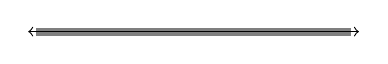
\begin{tikzpicture}
\draw[<->] (-2.1,0)--(2.1,0);
\xcoord{0}{c}
\draw[line width=1mm, opacity=0.5] (-2,0)--(2,0);
\end{tikzpicture}
\end{center}\pause
\item There is a number $0<R<\infty$ such that the series converges
for $|x-c|<R$ and diverges for $|x-c|>R$. Then $R$ is called the radius
of convergence.
\begin{center}
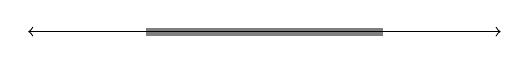
\begin{tikzpicture}
\draw[<->] (-3,0)--(3,0);
\xcoord{1.5}{c+R}
\xcoord{-1.5}{c-R}
\xcoord{0}{c}
\draw[line width=1mm, opacity=0.5] (-1.5,0)--(1.5,0);
\end{tikzpicture}
\end{center}\pause
\item The series converges for $x=c$ and diverges for all $x\ne c$.
In this case, we say that the radius of convergence is $0$.
\begin{center}
\begin{tikzpicture}
\draw[<->] (-2,0)--(2,0);
\xcoord{0}{c}
\draw(0,0)node[vertex]{};
\end{tikzpicture}
\end{center}
\end{enumerate}
\end{block}
\end{frame}
%----------------------------------------------------------------------------------------
\begin{frame}[t]
\AnswerYes<2>
\sStatusBar{3}{15}
\nsStatusBar{3}{13}
\nsMoreSpace<12>
\unote{Example~\eref{text}{eg:SRintervalA}}
We are told that a certain power series with centre $c=3$ converges
at $x=4$ and diverges at $x=1$. What else can we say about the
convergence or divergence of the series for other values of $x$?\medskip

\only<1|handout:0>{\MoreSpace
\fbox{\parbox{\textwidth}{\footnotesize
Given a power series (say with centre $c$), one of the
following holds.
\begin{enumerate}[(a)]
\item The power series converges for every number $x$. In this case we say that
the radius of convergence is $\infty$.
\begin{center}
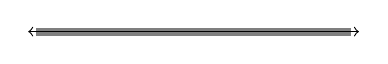
\begin{tikzpicture}
\draw[<->] (-2.1,0)--(2.1,0);
\xcoord{0}{c}
\draw[line width=1mm, opacity=0.5] (-2,0)--(2,0);
\end{tikzpicture}
\end{center}
\item There is a number $0<R<\infty$ such that the series converges
for $|x-c|<R$ and diverges for $|x-c|>R$. Then $R$ is called the radius
of convergence.
\begin{center}
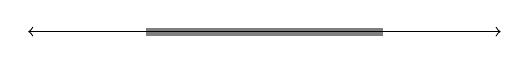
\begin{tikzpicture}
\draw[<->] (-3,0)--(3,0);
\xcoord{1.5}{c+R}
\xcoord{-1.5}{c-R}
\xcoord{0}{c}
\draw[line width=1mm, opacity=0.5] (-1.5,0)--(1.5,0);
\end{tikzpicture}
\end{center}
\item The series converges for $x=c$ and diverges for all $x\ne c$.
In this case, we say that the radius of convergence is $0$.
\begin{center}
\begin{tikzpicture}
\draw[<->] (-2,0)--(2,0);
\xcoord{0}{c}
\draw(0,0)node[vertex]{};
\end{tikzpicture}
\end{center}
\end{enumerate}
}}}

\color{spoilercolor}
\only<3-12|handout:0>{
From the theorem, we know that there is some real number $R$ such that the series converges when $|x-3|<R$ and diverges when $|x-3|>R.$

\begin{center}
\begin{tikzpicture}
\draw[<->] (-5,0)--(5,0);
\xcoord{0}{3}
\xcoord{1}{\stackrel{\text{converges}}{4}}
\xcoord{-2}{\stackrel{\text{diverges}}{1}}
\foreach \x in{1,...,9}{
	\ADD{3}{\x}{\s}
	\onslide<\s>{\MULTIPLY{\x}{.25}{\w}
	\ifdim \w pt < 1 pt
	\draw[line width=1mm, opacity=0.5,M5] (-\w,0)--(\w,0);
	\draw[M5,decorate,decoration={brace,amplitude=5pt}] (0,.3)--(\w,0.3)node[midway,above,yshift=2mm]{this $R$ is too small};
	\else
		\ifdim \w pt > 2 pt
		\draw[line width=1mm, opacity=0.5,W1] (-\w,0)--(\w,0);
		\draw[W1,decorate,decoration={brace,amplitude=5pt}] (0,.3)--(\w,0.3)node[midway,above]{this $R$ is too big};
		\else
		\draw[line width=1mm, opacity=0.5] (-\w,0)--(\w,0);
		\draw[C1,decorate,decoration={brace,amplitude=5pt}] (0,.3)--(\w,0.3)node[midway,above,yshift=1mm]{this $R$ is plausible};
	\fi\fi
}}
\end{tikzpicture}
\end{center}
\sonslide{\begin{itemize}\color{spoilercolor}
\item The series converges at $x=4$, so $|4-3|\not> R$, so $R \geq 1$.
\item The series diverges at $x=1$, so $|1-3|\not< R$, so $R \leq 2$.
\end{itemize}
So  for some number $1 \le R \le 2$, the series converges for $|x-3|<R$, and diverges for $|x-3|>R$.
}}
\only<13-|handout:0>{
\begin{center}
\begin{tikzpicture}
\draw[<->] (-5,0)--(5,0);
\xcoord{-2}{1}
\xcoord{-1}{2}
\xcoord{0}{3}
\xcoord{1}{4}
\xcoord{2}{5}

\sonslide<13->{\draw[line width=2mm, opacity=0.3,C1] (-1,0)--(1,0);}
\onslide<13-14>{\draw[C1,dashed] (1,0) arc (0:360:1cm);}
\sonslide<14->{\draw[line width=2mm, opacity=0.3,W1] (-5,0)--(-2,0) (2,0)--(5,0);}
\snshonslide{14}{13}{0}{\draw[W1,dashed] (2,0) arc (0:360:2cm);}
\end{tikzpicture}
\end{center}
\begin{itemize}\color{spoilercolor}
\item \snshonslide{13-}{13}{0}{\textcolor{C1}{ From $R \ge 1$, we know \sonslide{\textcolor{C1}{the series converges for $x$ in the interval $(2,4]$.}}}}
\item \snshonslide{14-}{13}{0}{ \textcolor{W1}{From $R \le 2$, we know \sonslide{\textcolor{W1}{the series diverges for $x$ in the $(-\infty,1] \cup (5,\infty)$.} }}}
\item \snshonslide{15-}{13}{0}{We do not know whether the series converges for other $x$.}
\end{itemize}}
\end{frame}
%----------------------------------------------------------------------------------------
%----------------------------------------------------------------------------------------
\section{3.5.2 Working with power series}
%----------------------------------------------------------------------------------------
%----------------------------------------------------------------------------------------
\begin{frame}[t,label=operations]
\StatusBar{1}{4}
\unote{Theorem~\eref{text}{thm:SRpsops}, abridged}
\begin{block}{Operations on Power Series}
Assume that the functions $f(x)$ and $g(x)$ are given by the power series
\centerline{
$f(x) = \sum\limits_{n=0}^\infty A_n (x-c)^n$ \qquad
$g(x) = \sum\limits_{n=0}^\infty B_n (x-c)^n$
}
for all $x$ obeying $|x-c|<R$. \only<1>{Let $K$ be a constant.} \only<-3>{ Then:}
\begin{align*}
\only<1|handout:1>{f(x)+g(x)   &= \sum_{n=0}^\infty [A_n+B_n]\, (x-c)^n \\
  Kf(x)     &= \sum_{n=0}^\infty K\, A_n\, (x-c)^n \\}
\only<2|handout:2>{(x-c)^Nf(x) &= \sum_{n=0}^\infty A_n\, (x-c)^{n+N}
                         \quad\text{for any integer $N\ge 1$}\\
           &= \sum_{k=N}^\infty A_{k-N}\, (x-c)^k
                         \quad\text{where $k=n+N$}\\}
\only<3|handout:3>{f'(x)     &= \sum_{n=0}^\infty A_n\, n\,(x-c)^{n-1}
           = \sum_{n=1}^\infty A_n\, n\,(x-c)^{n-1} \\
\int_c^x f(t)\ \dee{t} &= \sum_{n=0}^\infty A_n \frac{(x-c)^{n+1}}{n+1} \\
\int  f(x)\ \dee{x} &= \bigg[\sum_{n=0}^\infty A_n \frac{(x-c)^{n+1}}{n+1}\bigg]+C
\quad\text{with $C$ an arbitrary constant}}
\end{align*}
\only<-3>{for all $x$ obeying $|x-c|<R$.}


\only<4-|handout:4>{Differentiating, antidifferentiating, multiplying by a nonzero constant, and multiplying by a positive power of $(x-c)$ do not change the radius of convergence of $f(x)$ (although they may change the interval of convergence).}
\end{block}
\end{frame}
%----------------------------------------------------------------------------------------
%----------------------------------------------------------------------------------------
\begin{frame}[t]
\unote{Example~\eref{text}{eg:SRpsrepB}}
\AnswerSpace
\QuestionBar<1>{1}{4}\AnswerYes<1>
\AnswerBar<2->{1}{4}
Given that $\ds\diff{}{x}\left\{\frac{1}{1-x}\right\}=\frac{1}{(1-x)^2}$, find a power series representation for $\ds\frac{1}{(1-x)^2}$ when $|x|<1$.
\sonslide<2>{
For $|x|<1$:
\begin{align*}
\frac{1}{(1-x)^2}&=
\diff{}{x}\left\{\frac{1}{1-x}\right\}\\
&=
\diff{}{x}\left\{\sum_{n=0}^\infty x^n
\right\}\\
&=\sum_{n=0}^\infty \left(\diff{}{x}\left\{x^n\right\} \right)\\
&=\sum_{n=0}^\infty nx^{n-1}\\
&=\sum_{n=1}^\infty nx^{n-1}
\end{align*}
}

\end{frame}
%----------------------------------------------------------------------------------------
\begin{frame}[t]
\unote{Example~\eref{text}{eg:SRpsrepC}}
\QuestionBar<1>{2}{4}\AnswerYes<1>
\AnswerBar<2->{2}{4}
Find a power series representation for $\log(1+x)$ when $|x|<1$.
\vfill
\sonly<2>{
First, note $\diff{}{x}\{\log(1+x)\}=\frac{1}{1+x}$.
Our plan is to antidifferentiate a power series representation of $\frac{1}{1+x}$.
For $|x|<1$:
\begin{align*}
\frac{1}{1+x}&=\frac{1}{1-(-x)}=\sum_{n=0}^\infty (-x)^n=\sum_{n=0}^\infty (-1)^nx^n\\
\int \frac{1}{1+x}\,\dee x & =\int\left(\sum_{n=0}^\infty (-1)^nx^n\right)\,\dee x\\
&=\sum_{n=0}^\infty \left(\int(-1)^nx^n\,\dee x\right)
\intertext{So, for some constant $C$,}
\log(1+x)&=C+\sum_{n=0}^\infty (-1)^n\frac{x^{n+1}}{n+1}=C+\sum_{n=1}^\infty (-1)^{n+1}\frac{x^n}{n}
\end{align*}
}
\sonly<3>{
To find $C$, let's plug in a value for $x$ where both sides of the equation are easy to evaluate: $x=0$.
\begin{align*}
\log(1+0)&=C+\sum_{n=1}^\infty (-1)^{n+1}\frac{0^{n}}{n}\\
0&=C\\
\text{So, }
\log(1+x)&=\sum_{n=1}^\infty (-1)^{n+1}\frac{x^n}{n}
\end{align*}
when $|x|<1$.}
\end{frame}
%----------------------------------------------------------------------------------------
\begin{frame}[t]
\unote{Example~\eref{text}{eg:SRpsrepD}}
\AnswerYes<1-2>
\QuestionBar<1>{3}{4}
\AnswerBar<2->{3}{4}
Find a power series representation for $\arctan(x)$ when $|x|<1$.
\vfill
\sonly<2>{
First, note $\diff{}{x}\left\{\arctan x\right\}=\frac{1}{1+x^2}$. To obtain a power series representation of $\frac{1}{1+x^2}$, we'll 
substitute into the geometric series. 

Let $y=-x^2$ with $|y|<1$. Then:
\begin{align*}
\frac{1}{1-y}&=\sum_{n=0}^\infty y^n\\
\implies \frac{1}{1+x^2}&=\sum_{n=0}^\infty {(-x^2)}^n=\sum_{n=0}^\infty(-1)^nx^{2n}\\
\implies \int\frac{1}{1+x^2}\, \dee x&=\int\left(\sum_{n=0}^\infty(-1)^nx^{2n}\right)\,\dee x=\sum_{n=0}^\infty\left(\int(-1)^nx^{2n}\,\dee x\right)\\
\implies \arctan x & = C+\sum_{n=0}^\infty (-1)^n\frac{x^{2n+1}}{2n+1}
\end{align*}
for some constant $C$.
}
\sonly<3>{
To find $C$, we'll plug in $x=0$, which makes both sides of the last equation easy to evaluate.
\begin{align*}
\arctan 0 & = C+\sum_{n=0}^\infty (-1)^n\frac{x^{2n+1}}{2n+1}\\
0&=C\\
\text{So, } \arctan x & = \sum_{n=0}^\infty (-1)^n\frac{x^{2n+1}}{2n+1}
\end{align*}
when $|-x^2|<1$, i.e. when $|x|<1$.
}
\end{frame}
%----------------------------------------------------------------------------------------
\begin{frame}[t]
\unote{Theorem~\eref{text}{thm:SRpsSub}}
\begin{block}{Substituting in a Power Series}
Assume that the function $f(x)$ is given by the power
series
\begin{equation*}
f(x) = \sum_{n=0}^\infty A_n x^n
\end{equation*}
for all $x$ in the interval $I$. Also let $K$ and $k$ be real constants. Then
\begin{align*}
f\big(Kx^k\big)   &= \sum_{n=0}^\infty A_nK^n\, x^{kn} \\
\end{align*}
whenever $Kx^k$ is in $I$. In particular, if $\sum_{n=0}^\infty A_n x^n$
has radius of convergence $R$, $K$ is nonzero and $k$ is a natural number,
then $\sum_{n=0}^\infty A_nK^n\, x^{kn}$ has radius of convergence
$\root{k}\of{R/|K|}$.
\end{block}

\end{frame}
%----------------------------------------------------------------------------------------
%----------------------------------------------------------------------------------------
\begin{frame}[t]
\unote{Example~\eref{text}{eg:SRpsrepAAA}}
\AnswerYes<1-2>
\QuestionBar<1>{4}{4}
\AnswerBar<2->{4}{4}
Find a power series representation for $\dfrac{1}{5-x}$ with centre 3.
\vfill
\sonly<2>{
We know that $\frac{1}{1-(x-3)}=\sum_{n=0}^\infty (x-3)^n$ when $|x-3|<1$. To take advantage of our ability to substitute into power functions, 
we'd like to write $\frac{1}{5-x}$ in the form $\frac{1}{1-K(x-3)^k}$ for some constant $K$ and some whole number $k$.
\begin{align*}
\frac{1}{5-x}&=\frac{1}{2-(x-3)}=\frac12\cdot\frac{1}{1-\left(\frac{x-3}{2}\right)}
\intertext{Set $y=\frac{x-3}{2}$. When $|y|<1$:}
\frac12\cdot \frac{1}{1-y}&=\frac{1}{2}\sum_{n=0}^\infty y^n\\
\implies
\frac12\cdot\frac1{1-\left(\frac{x-3}{2}\right)}&=\frac12\sum_{n=0}^\infty \left(\frac{x-3}{2}\right)^n\\
\implies \frac{1}{5-x}&=\sum_{n=0}^\infty \frac{(x-3)^n}{2^{n+1}}.
\end{align*}
}
\sonly<3>{The series converges when:
\begin{align*}
|y|&<1\\
\left|\frac{x-3}{2}\right|&<1\\
|x-3|&<2
\end{align*}
So the radius of convergence of our series is 2.}
\end{frame}
%----------------------------------------------------------------------------------------
%----------------------------------------------------------------------------------------
%----------------------------------------------------------------------------------------
%----------------------------------------------------------------------------------------
